\documentclass[a4paper]{article}


\usepackage[T1]{fontenc}    
\usepackage[utf8]{inputenc} 
\usepackage{textcomp}      
\date{} 					
\author{}                   
\usepackage{geometry}		
\geometry{ left=2cm, right=2cm, top=2cm, bottom=4cm, bindingoffset=5mm}

\usepackage{graphicx}
\usepackage{xcolor}
\usepackage{hyperref} 
\usepackage{fancyhdr}
\usepackage{amsmath}											
\pagestyle{fancy}
\fancyhf{}
\fancyhead[R]{2973140 - Felix Bühler  \\ 2893121 - Jan Leusmann \\  3141241 - Jamie Ullerich}
\fancyhead[L]{Scientific Visualisation \\ Sommersemester 2019 }
\renewcommand{\headrulewidth}{0.5pt} 				

\title{Exercise 7}

\begin{document}

\maketitle 
\thispagestyle{fancy}


\section*{Exercise 7.1 - Glyphs}
\begin{enumerate}
	\item[Design a)]
		Humans can recognize patterns and textures, and this approach can illustrate 12 different attributes. 
		The attributes are displayed via thickness, length and angle of the lines which may be easy to distinguish if there is a great difference but not if there is little difference. 
		So these glyphs are rather difficult to interpret, but would explain facts of the car scenario. 
	\item [Design b)]
		Distances are hard to judge, especially if there is a small distance. 
		Besides that, these glyphs are easier to compare since all attributes are always at the same place.
		This visualisation would be appropriate for the car scenario. 	
	\item[Design c)]
		Some features may be easier to perceive than others, for example the head eccentricity is easier to distinguish than the nose length or mouth curvature. 
		But in general, humans are capable of recognizing different faces. 
		This can encode all 12 attributes, as well. 
		Therefore, it is possible to describe the car scenario but not as easy to read as the star plots. 
	\item[Design d)]
		The advantage of these glyphs is that they can visualise time dependent flows, but this is not important in the described scenario. 
		Therefore, this glyph design is not suitable for the car scenario. 
\end{enumerate}

\newpage
\section*{Exercise 7.2 - Isolines}

\begin{enumerate}
	\item[1:] calculate function values according to formula \\
	 
				$f(-1.5, 1.5) = (-1.5 - 0.5)^{2} - 1.5^{2} =$ 1.75 = 1.8\\
				$f(-0.5, 1.5) =$ -1.25 = -1.3\\
				$f(0.5, 1.5) =$ -2.25 = -2.3\\
				$f(1.5, 1.5) =$ -1.25 = -1.3\\
				$f(-1.5, 0.5) =$ 3.75 = 3.8\\
				$f(-0.5, 0.5) =$ 0.75 = 0.8\\
				$f(0.5, 0.5) =$ -0.25 = -0.3\\
				$f(1.5, 0.5) =$ 0.75 = 0.8\\
				$f(-1.5, -0.5) =$ 3.75 = 3.8\\
				$f(-0.5, -0.5) =$ 0.75 = 0.8\\
				$f(0.5, -0.5) =$ -0.25 = -0.3\\
				$f(1.5, -0.5) =$ 0.75 = 0.8 \\
				$f(-1.5, -1.5) =$ 1.75 = 1.8 \\
				$f(-0.5, -1.5) =$ -1.25 = -1.3\\
				$f(0.5, -1.5) =$ -2.25 = -2.3\\
				$f(1.5, -1.5) =$ -1.25 = -1.3\\
				
				\begin{figure}[h!]
					\centering 
					\includegraphics[width=11cm]{7_2_1.png}
					\caption{coordinates and function values }
					\label{fig:coordinates}
				\end{figure}
	\newpage
	\item[2:] mark nodes depending on condition
			\begin{figure}[h!]
				\centering 
				\includegraphics[width=11cm]{7_2_2.png}
				\caption{intersected lines: violet}
				\label{}
			\end{figure}
		
	\item[2:] find position of intersection on edge by linear interpolation \\
		
			$x = \dfrac{(f_{2} - c) \cdot x_{1} + (c - f_{1}) \cdot x_{2}}{(f_{2} - f_{1})}$\\
			
			%$f_{1} = 1.8; f_{2} = -1.3; x_{1} = -1.5; x_{2} = -0.5$\\
			$ x_{1} = \dfrac{(-1.3 - 0) \cdot -1.5 + (0 - 1.8) \cdot -0.5}{(-1.3 - 1.8)} = \dfrac{1.95 + 0.9}{-3.1} = -0.91935$\\ 
			
			%$x_{2} = \dfrac{(0.8 - 0) \cdot -0.5 + (0 - - 1.3) \cdot -0.5}{(0.8 - -1.3)} = \dfrac{-1.05 + 0.9}{2.1} = -0.5$\\
			$y_{2} = \dfrac{(0.8 - 0) \cdot 1.5 + (0 + 1.3) \cdot 0.5}{(0.8 + 1.3)} = \dfrac{1.85}{2.1} = 0.881$\\
			
			$x_{3} = \dfrac{(-0.3 - 0) \cdot -0.5 + (0 - 0.8) \cdot 0.5}{(-0.3 - 0.8)} = \dfrac{-0.25}{-1.1} = 0.227$\\
			
			$x_{4} = \dfrac{(0.8 - 0) \cdot 0.5 + (0 + 0.3) \cdot 1.5}{(0.8 + 0.3)} = \dfrac{0.85}{1.1} =  0.773 $\\ 
			
			$y_{5} = \dfrac{(0.8 - 0) \cdot 1.5 + (0 + 1.3) \cdot 0.5}{(0.8 + 1.3)} = \dfrac{1.85}{2.1} = 0.881$\\
			
			$x_{6} = \dfrac{(-0.3 - 0) \cdot -0.5 + (0 - 0.8) \cdot 0.5}{(-0.3 - 0.8)} = \dfrac{-0.25}{-1.1} = 0.227$\\
			
			$x_{7} = \dfrac{(0.8 - 0) \cdot 0.5 + (0 + 0.3) \cdot 1.5}{(0.8 + 0.3)} = \dfrac{0.85}{1.1} =  0.773 $\\ 
			
			$ x_{8} = \dfrac{(-1.3 - 0) \cdot -1.5 + (0 - 1.8) \cdot -0.5}{(-1.3 - 1.8)} = \dfrac{1.95 + 0.9}{-3.1} = -0.91935$\\ 
			
			$y_{9} = \dfrac{(-1.3 - 0) \cdot -0.5 + (0 - 0.8) \cdot -1.5}{(- 1.3 - 0.8)} = \dfrac{1.85}{- 2.1} = - 0.881$\\


			$y_{10} = \dfrac{(-1.3 - 0) \cdot -0.5 + (0 - 0.8) \cdot -1.5}{(- 1.3 - 0.8)} = \dfrac{1.85}{- 2.1} = - 0.881$\\	
			
					
			\begin{figure}[h!]
				\centering 
				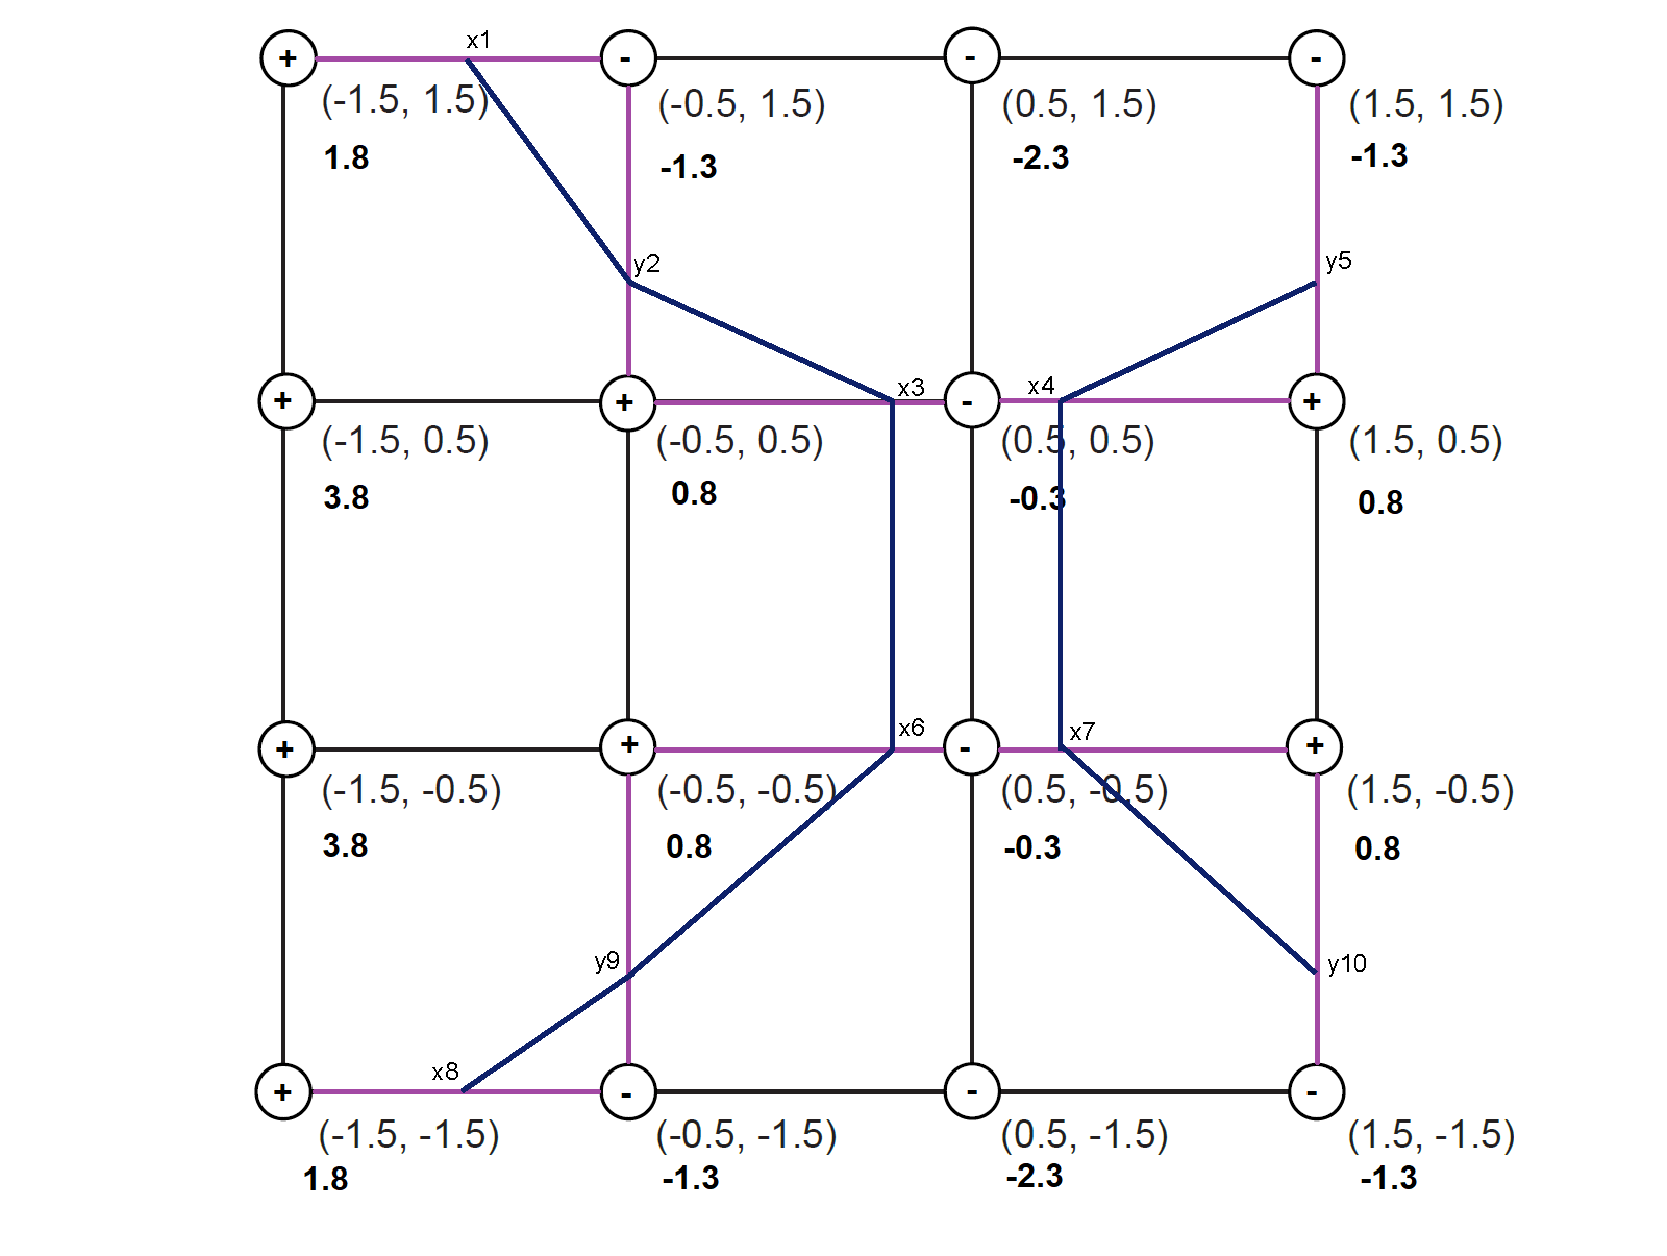
\includegraphics[width=13cm]{7_2_2_2.pdf}
				\caption{isolines: blue}
				\label{}
			\end{figure}
			
\end{enumerate}





\end{document}